%! suppress = Quote


\section{Анализ предметной области}

В данной главе будет дан обзор системы типов языка Kotlin, на прикладных примерах описаны некоторые ограничения её выразительности и доступные решения.
После будет введено понятие Self-типа и показаны его преимущества как потенциального решения обозначенных проблем.
В завершение будут приведены приложения Self-типов в других задачах.

Для нашего изложения не принципиальна аккуратная формализация понятий объекта, наследования, подтипизации, полиморфизма с ограничениями и д.р.
Они будут даны прикладным образом как описание релевантных данной работе возможностей языка Kotlin.
Однако некоторые формализмы будут введены в разделе~\ref{subsec:formalizaton} для демонстрации особенностей Self-типов, которые могут приводить к небезопасности системы типов (опр.~\ref{def:sound}).
В данной работе не ставится задачи формального доказательства безопасности, но встраивание в систему типов языка Kotlin новой возможности заведомо безопасным образом (в соответствии с существующими результатами, приведёнными в~\ref{subsec:formal-solutions}), покрывая релевантные случаи использования, данные в~\ref{subsec:applications}.


\subsection{Система типов языка Kotlin}

\term{Kotlin} --- это объектно-ориентированный промышленный язык программирования, поддерживающий компиляцию в Java bytecode, JavaScript и нативный код~\cite{jemerov2017kotlin}.

\begin{definition}
    \term{Система типов} --- это гибко управляемый синтаксический метод доказательства отсутствия в программе определенных видов поведения при помощи классификации выражений языка по разновидностям вычисляемых ими значений~\cite{pierce2002types}.
\end{definition}

\begin{definition}
    \label{def:subtype}
    Тип \texttt{B} является \term{подтипом} типа \texttt{A} (\texttt{A} в таком случае~--- \term{надтип} \texttt{B}), если произвольное выражение типа \texttt{B} может быть безопасно использовано в позиции, в которой ожидается выражение типа \texttt{A}~\cite{liskov1987keynote, pierce2002types}.
    Обозначение \texttt{B <: A}.
    Если два типа \texttt{C} и \texttt{D} не связаны отношением подтипизации, это обозначается так: \texttt{C !<:> D}.
\end{definition}

Система типов языка программирования Kotlin обладает следующими основными свойствами~\cite{akhin2021kotlin}.
\begin{itemize}
    \item Статическая --- проверка типов происходит на этапе компиляции;
    \item Gradual~\cite{siek2007gradual} --- система типов может накладывать более слабые ограничения, делегируя проверку типов времени исполнения программы для лучшей поддержки взаимодействия с кодом целевой платформы (реализуется в Kotlin с помощью \term{flexible types});
    \item Flow~\cite{pearce2013calculus} --- типизация значений в программе может зависеть от графа потока управления (реализуется в Kotlin через механизм \term{smart-casts}, см.~\ref{subsubsec:smart-casts});
    \item Null-безопасная --- вводится две вселенные типов: типы, которые содержат значение \mintinline{kotlin}|null| (обозначаются знаком вопроса в конце записи типа), и которые \mintinline{kotlin}|null| не содержат;
    \item Без небезопасных неявных типовых конверсий;
    \item С поддержкой параметрического полиморфизма (опр.~\ref{def:param-poly}) с ограничениями (\ref{subsubsec:variance});
    \item С номинальной подтипизацией --- один тип является подтипом (опр.~\ref{def:subtype}) другого только в случае явного указания программиста в виде наследования (\ref{subsubsec:interitance-virtual}) или вариантности типовых параметров (\ref{subsubsec:variance});
    \item С общими верхним и нижним типами относительно отношения подтипизации --- тип \mintinline{kotlin}|Nothing| является подтипом любого типа, а \mintinline{kotlin}|Any?| --- супертипом любого типа.
\end{itemize}

\subsubsection{Наследование и виртуальный полиморфизм} \label{subsubsec:interitance-virtual}

Система типов языка Kotlin является \term{номинативной}.
Это значит, что отношение подтипизации нужно указывать явно и оно не следует из структуры значений типа.
Основным способом задания отношения подтипизации в Kotlin является \term{наследование}.

С помощью наследования же в Kotlin реализуется \term{виртуальный полиморфизм}.
Он заключается в том, что по ссылке базового типа происходит вызов метода наследника, если в действительность это ссылка на объект наследника.
\begin{minted}{kotlin}
    open class Base {
        fun method() { println("Base") }
    }

    class Derived : Base() {
        override fun method() { println("Derived") }
    }

    fun test() {
        val base: Base = Derived()
        base.method() // Печатает "Derived"
    }
\end{minted}

\subsubsection{Smart-casts}\label{subsubsec:smart-casts}

\begin{definition}
    \label{def:basic-block}
    \term{Базовый блок} --- непрерывная последовательность инструкций, всегда выполняющихся последовательно.
\end{definition}

\begin{definition}
    \label{def:cfg}
    \term{Граф потока управления программы (CFG --- control flow graph)} --- граф, составленный по программе из её базовых блоков.
    На рисунке~\ref{fig:cfg-example} приведён пример графа потока управления.
\end{definition}

\begin{figure}
    \centering
    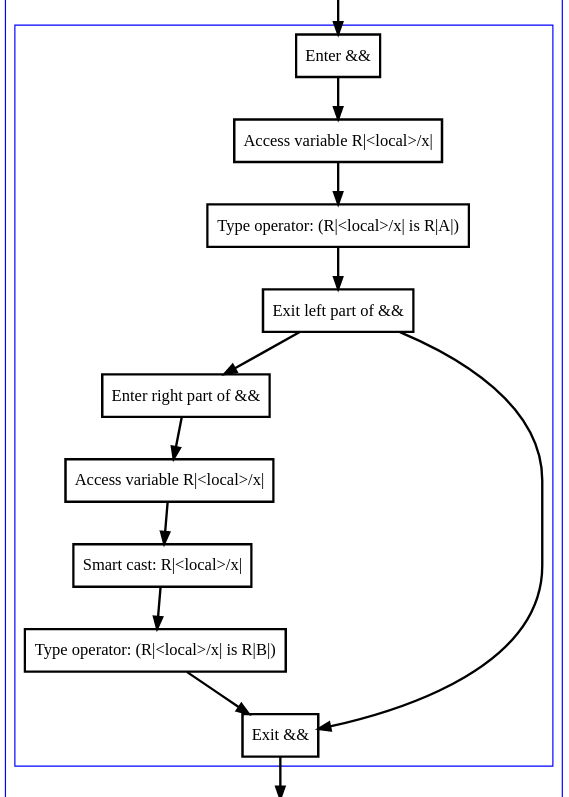
\includegraphics[width=0.8\linewidth]{fig/cfgExample}
    %! suppress = EscapeAmpersand
    \caption{Граф потока управления выражения \mintinline{kotlin}|x is A && x is B|.}
    \label{fig:cfg-example}
\end{figure}

\begin{definition}
    \label{def:intersection-types}
    \term{Тип-пересечение} --- тип, являющийся подтипом одновременно всех типов из пересечения.
    Обозначение для пересечения типов \texttt{A}, \texttt{B} и \texttt{C}: \texttt{A \& B \& C}.
\end{definition}

Типы-пересечения являются примером типов, которые нельзя записать в Kotlin, то есть они не доступны программисту, но возникают в процессе вывода типов.
\begin{minted}{kotlin}
    interface A {
        fun aMethod() { /* ... */ }
    }

    interface B {
        fun bMethod() { /* ... */ }
    }

    class C : A, B
    class D : A, B

    fun test(cond: Boolean) {
        val intersection /* : A & B */ = if (b) C() else D()
        intersection.aMethod() // ok
        intersection.bMethod() // ok
    }
\end{minted}

\begin{definition}
    \term{Smart-casts} --- механизм уточнения типа за счёт информации, получаемой из графа потока управления программы.
\end{definition}

Например, если в условной конструкции проверяется принадлежность значения переменной типу, то в теле доступна информация о том, что тип этой переменной включает в себя тип из условия.
Это выражается с помощью типов-пересечений (опр.~\ref{def:intersection-types}).

\begin{minted}{kotlin}
    fun test(x: A) {
        if (x is B) {
            // x: A & B
            #\colorbox{green}{x}#.bMethod()
        }
    }
\end{minted}

\subsubsection{Параметрический полиморфизм и вариантность}\label{subsubsec:variance}

\begin{definition}
    \label{def:param-poly}
    \term{Параметрический полиморфизм} --- способность функции или класса работать с объектами различных типов путём абстрагирования реализации по \term{типовому параметру}.
    Тип, подставляемый вместо типового параметра~--- \term{типовой аргумент}.
\end{definition}

\begin{definition}
    \term{Параметрический полиморфизм с поддержкой ограничений}~--- параметрический полиморфизм, поддерживающий добавление ограничений на типы, которые можно использовать как типовые аргументы.
    В случае Kotlin, данным ограничением является требование на наличие у типа определённого супертипа.
\end{definition}

\begin{definition}
    \label{def:variance}
    \term{Вариантность} --- механизм языков с параметрическим полиморфизмом, позволяющий дополнять отношение подтипизации между параметризованными типами, когда типовые аргументы --- разные типы, связанные в свою очередь отношением подтипизации.
\end{definition}

В Kotlin вариантность может сообщаться как типовому параметру класса, так и в месте использования этого класса.
В нашем изложении мы ограничимся только первым случаем, второй рассматривается аналогично.

\begin{definition}
    \label{def:type-positions}
    Возвращаемый тип функции будем называть типом в \term{исходящей позиции}.
    Тип параметра функции будем называть типом во \term{входящей позиции}.
    Тип, выступающий ковариантным типовым аргументом типа во входящей позиции, будем называть типом во \emph{входящей ковариантной позиции}.
    Аналогично для исходящей позиции и других вариантностей.
\end{definition}

\begin{definition}
    \label{def:type-position-sign}
    Типом в \term{положительной или ковариантной позиции} будем называть тип в исходящей позиции, исходящей ковариантной позиции или входящей контравариантной позиции\footnote{Определение типовых позиций даётся с практической точки зрения и не с самом общем случае, но достаточном для данного изложения.}.
    Типом в \term{отрицательной или контравариантной позиции} будем называть тип во входящей позиции, во входящей ковариантной позиции и в исходящей контравариантной позиции.
\end{definition}

\begin{definition}
    \label{def:invariant}
    \term{Инвариантный типовой параметр} --- может использоваться в произвольных позициях деклараций методов класса.
    Не дополняет отношение подтипизации между параметризованными типами.
\end{definition}

\begin{minted}[escapeinside=??,mathescape]{kotlin}
    interface Inv<T> {
        fun id(x: ?\framebox{T}?): ?\framebox{T}?
    }

    // $\forall$A, B. Inv<A> !<:> Inv<B>
    fun test(b: Inv<B>) {
        // Отношение подтипизации не задано
        val a: Inv<A> = b // ошибка компиляции
    }
\end{minted}

\begin{definition}
    \label{def:covariant}
    \term{Ковариантный типовой параметр} --- может использовать в положительных позициях деклараций методов класса.
    Параметризованный тип образует такое же отношение подтипизации, что и типовые аргументы.
\end{definition}

\begin{minted}[escapeinside=??]{kotlin}
    interface Out<?\framebox{out}? T> {
        fun produce(): ?\framebox{T}?
    }

    // B <: A <=> Out<B> <: Out<A>
    fun test(b: Inv<B>) {
        val a: Inv<A> = b
    }
\end{minted}

\begin{definition}
    \label{def:contravariant}
    \term{Контравариантный типовой параметр}~--- может использоваться в отрицательных позициях деклараций методов класса.
    Параметризованный тип образует обратное отношение подтипизации относительно типовых аргументов.
\end{definition}

\begin{minted}[escapeinside=??]{kotlin}
    interface In<?\framebox{in}? T> {
        fun consume(x: ?\framebox{T}?)
    }

    // B <: A <=> In<A> <: In<B>
    fun test(a: Inv<A>) {
        val b: Inv<B> = b
    }
\end{minted}

\subsubsection{Ресиверы в Kotlin}

\begin{definition}
    \label{def:receivers}
    Каждая функция, объявленная как метод или функция-расширение имеет специальные параметры (один или более), называемые \term{ресиверами}~\cite{akhin2021kotlin}.
    Такие параметры доступны как \mintinline{kotlin}|this| в теле функции.
\end{definition}

Далее в зависимости от контекста будем произвольно называть ресиверами такие специальные параметры, а так же объекты, используемые как соответствующие этим параметрам аргументы.
Например, в вызове \mintinline{kotlin}|"a".plus("b")| строка \mintinline{kotlin}|"a"| является объектом-ресивером для функции \mintinline{kotlin}|plus|.

Ресиверы в Kotlin могут быть трёх видов: dispatch, extension и context-ресиверы.

\begin{definition}
    \label{def:dispatch-receivers}
    \term{Dispatch-ресивер} --- ресивер, по которому происходит виртуальная диспетчеризация вызова.
\end{definition}

\begin{minted}[escapeinside=??]{kotlin}
    interface Base {
        fun greet()
    }

    class Derived : Base {
        override fun greet() {
            println("Hello")
        }
    }

    val b: Base = Derived();
    // b - dispatch-ресивер вызова
    b.greet() // Печатает "Hello"
\end{minted}

\begin{definition}
    \label{def:extension-receivers}
    \term{Extension-ресивер} --- ресивер, который является лишь специальным аргументом функции, но по которому не происходит виртуальной диспетчеризации вызова.
\end{definition}

\begin{minted}{kotlin}
    fun String.twice() = this + this
    // функционально аналогично определению
    // fun twice(String s) = s + s

    println("Y".twice()) // Печатает "YY"
\end{minted}

\begin{definition}
    \label{def:context-receivers}
    \term{Context-ресивер} --- ресивер, аналогичный extension-ресиверу (опр.~\ref{def:extension-receivers}), только для него не доступен синтаксис вызова функции явно через точку (не может быть явным).
\end{definition}

В дальнейшем изложении если не уточняется вид ресивера, имеется в виду dispatch или extension ресивер.

\subsubsection{Типовые скоупы}

\begin{definition}
    \label{def:type-scope}
    \term{Типовой скоуп}~--- множество функций, для которых объект данного типа может быть использован как ресивер.
\end{definition}

Например, функция \mintinline{kotlin}|plus| содержится с скоупе типа \mintinline{kotlin}|String|: \\\mintinline{kotlin}|(plus: String.(String) -> String)| $\in$ \mintinline{kotlin}|scope(String)|.


\subsection{Описание проблемы и возможных решений}

Рассмотрим следующую задачу.
Допустим, требуется в типе функции выразить, она возвращает тип, совпадающий с типом ресивера, на котором она вызвана (это может быть тот класс, в котором функция определена, либо его наследник).
В качестве примера рассмотрим потенциальные интерфейсы библиотеки персистентных коллекций.

\subsubsection{Рекурсивные дженерики} \label{subsubsec:recursive-generics}

Во-первых, требуемого можно добиться с помощью ковариантных типовых параметров с рекурсивными ограничениями --- \term{рекурсивных дженериков}.
Так, метод \texttt{add} должен вернуть новую коллекцию того же типа, но с добавленным элементом.
Обозначим это так, что \texttt{add} возвращает типовой параметр, который представляет собой конкретного наследника этого интерфейса, на котором вызывается метод.

\begin{minted}[escapeinside=??]{kotlin}
    interface PCollection<out E, ?\framebox{out S : PCollection<E, S>}?> {
        fun add(value: @UnsafeVariance E): ?\framebox{S}?
    }

    interface PList<out E, ?\framebox{out S : PList<E, S>}?> : PCollection<E, ?\framebox{S}?> {
        fun listSpecific()
    }

    class PListImpl<out E> : PList<E, ?\framebox{PListImpl<E>}?> {
        /* ... */
    }

    fun <T, ?\framebox{L}?> test(xs: ?\framebox{L}?, x: T) where ?\framebox{L : PList<T, L>}? {
        xs.add(x) /* : ?\framebox{L}? */ .listSpecific()
    }
\end{minted}

Видим, что паттерн рекурсивного ограничения распространяется по всему коду.
Также, в случае определения метода в любом месте иерархии кроме финального класса, требуется явное приведение типов: \mintinline[escapeinside=??]{kotlin}|this as S|.
Более того, такой подход является нетривиальным для понимания особенно начинающими разработчиками.

\subsubsection{Abstract override методы} \label{subsubsec:abstract-override}

Альтернативой может быть использование \term{abstract override методов}.
Теперь дополнительный типовой параметр не требуется, однако в каждом наследнике нужно добавить переопределяющий метод с более специфичным возвращаемым типом.

\begin{minted}[escapeinside=??]{kotlin}
    interface PCollection<out E> {
        fun add(value: @UnsafeVariance E): ?\framebox{PCollection<E>}?
    }

    interface PList<out E> : PCollection<E> {
        abstract override fun add(value: @UnsafeVariance E): ?\framebox{PList<E>}?
        fun listSpecific()
    }

    class PListImpl<out E> : PList<E> {
        /* ... */
    }

    fun <T> test(xs: PList<T>, x: T) {
        xs.add(x) /* : ?\framebox{PList<T>}? */ .listSpecific()
    }
\end{minted}

Видим, что теперь паттерн рекурсивного ограничения исчез, однако добавилась вспомогательная декларация.
У такого подхода можно выделить следующие недостатки.

\begin{itemize}
    \item Подобные декларации с более специфичными возвращаемыми типами требуется написать в теле каждого наследника, что приводит к существенному количеству шаблонного кода.
    \item Нет контроля со стороны компилятора, что программист не забыл добавить подобные декларации во всех наследников при добавлении нового метода в базовый класс, что особенно чувствительно для разработчиков библиотек.
    \item Этот подход имеет место только для возвращаемых типов, типы параметров методов же должны совпадать по правилу переопределения функций базовых классов.
\end{itemize}

Несмотря на обширный список недостатков, подход с abstract override методами используется, например, в библиотеке персистентных коллекций языка Kotlin \texttt{kotlinx.collection.immutable}\footnote{\url{https://github.com/Kotlin/kotlinx.collections.immutable}}.

\subsubsection{Ассоциированные типы}

\begin{definition}
    \label{def:assoc}
    \term{Ассоциированные типы}~\cite{chakravarty2005associated} --- это возможность объявить в базовом классе тип, определение которого будет дано только в реализации.
\end{definition}

Ассоциированные типы присутствуют в большом количестве языков без наследования, реализующих специальный полиморфизм через классы типов или трейты, например, Haskell и Rust.
Однако среди языков с наследованием ассоциированные типы встречаются не часто, например, в Swift и Scala.

Рассмотрим пример использования ассоциированных типов для интерфейсов персистентных коллекций на языке Scala, где ассоциированные типы носят название \term{abstract type members}\footnote{\url{https://docs.scala-lang.org/tour/abstract-type-members.html}}.

\begin{minted}{scala}
    trait PCollection[T] {
      #\framebox{type S}#
      def add(x: T): #\framebox{S}#
    }

    trait PList[T] extends PCollection[T] {
      #\framebox{type S <: PList[T]}#
      def listSpecific: Unit
    }

    class PListImpl[T] extends PList[T] {
      #\framebox{type S = PListImpl[T]}#
      override def add(x: T): #\framebox{PListImpl[T]}# = // ...
      override def listSpecific: Unit = // ...
    }
\end{minted}

Обозначим основные недостатки данного подхода.

\begin{itemize}
    \item Заметим, что аналогично подходу с abstract override методами в каждом абстрактном наследнике требуется уточнить ассоциированный тип.
    \item Так же нет контроля со стороны компилятора, что это утонение не было забыто.
    \item Определение ассоциированного типа должно быть дано либо в абстрактном классе, либо в первом не абстрактном классе в иерархии.
    Дальнейшее уточнение ассоциированного типа ниже по иерархии наследования невозможно.
    \item В реализациях методов, находящихся выше по иерархии наследования, чем определение ассоциированного типа, требуется явное приведение типов.
\end{itemize}

Более того, реализация ассоциированных типов в языке с наследованием является очень нетривиальной задачей, так как нельзя полагаться, что тип, ассоциированный с одним значением равен типу, ассоциированному с другим.
Поэтому приходится отслеживать, откуда пришло значение ассоциированного типа, и вместо установления подтипизации между двумя типами, сравнивать пути получения значений (значение может глубоко вложено как поле в композиции объектов).

Стоит отметить, что на момент написания данной работы запроса от пользователей на добавление ассоциированных типов в Kotlin нет.


\subsection{Self-типы} \label{subsec:self-types}

\begin{definition}
    \label{def:self-type}
    \term{Self-тип} --- тип ресивера (опр.~\ref{def:receivers}), на котором вызывается функция (тип \mintinline{kotlin}|this|'а).
\end{definition}

Self-типы в встречаются так же под названиями \term{рекурсивные типы}~\cite{amadio1993subtyping} и \term{This-типы} (\texttt{ThisType} в литературе~\cite{ryu2016thistype}).
А под названием Self-типы может подразумеваться нечто совершенно другое, как, например, в языке Scala\footnote{\url{https://docs.scala-lang.org/tour/self-types.html}}.

Рассмотрим следующий пример.
Пусть у нас есть базовый класс, в котором объявлен метод с \texttt{Self} в качестве возвращаемого типа.
Тогда при вызове этого метода базового класса на объекте наследника, мы сможем воспользоваться результатом как объектом типа наследника.

\begin{minted}[escapeinside=??]{kotlin}
interface Base {
    fun base(): ?\framebox{Self}? = ?\framebox{this}?
}

class Defived : Base {
    fun derived() { /* ... */ }
}

fun test(d: Derived) = d.base() /* : ?\framebox{Derived}? */ .derived()
\end{minted}

\begin{definition}
    \label{def:materialization}
    \term{Материализация Self-типа} --- подмена Self-типа в сигнатуре метода на тип ресивера в скоупе типа этого ресивера.
\end{definition}

Так для примера выше \texttt{Self} материализуется в \texttt{Derived} в его скоупе: \\
\mintinline[escapeinside=??]{kotlin}{(base: Base.() -> ?\framebox{Derived}?)} $\in$ \texttt{scope(Derived)}

\begin{definition}
    \label{def:bound}
    \term{Bound Self-типа} --- наиболее общий тип, в который Self-тип может быть материализован.
\end{definition}

Bound Self-типа совпадает с типом ресивера текущей декларации.
В примере выше для \mintinline[escapeinside=??]{kotlin}|?\framebox{Self}?| bound'ом является \mintinline{kotlin}|Base| (обозначение \underline{\mintinline{kotlin}|Self(Base)|}).

Вернёмся к примеру интерфейсов библиотеки персистентных коллекций (стр.~\pageref{subsubsec:recursive-generics} и~\pageref{subsubsec:abstract-override}).
Легко видеть, что вариант с Self-типами лишен перечисленных ранее недостатков.

\begin{minted}[escapeinside=??]{kotlin}
interface PCollection<out E> {
    fun add(value: @UnsafeVariance E): ?\framebox{Self}?
}

interface PList<out E> : PCollection<E> {
    fun listSpecific()
}

class PListImpl<out E> : PList<E> {
    /* ... */
}

fun <T> test(xs: PList<T>, x: T) {
    xs.add(x) /* : ?\framebox{PList<T>}? */ .listSpecific()
}
\end{minted}

Как было показано выше, Self-типы могут быть эмулированы с помощью нетривиального кода с рекурсивными дженериками, дополнительными явными приведениями типов и некоторого количества boilerplate code.
Однако, как мы покажем в разделе (\ref{subsec:applications}), Self-типы оказываются полезны для реализации нескольких популярных шаблонов программирования.
Отсутствие Self-типов в языке и сложность их эмуляции может в некоторых случаях заставлять принимать менее удачные решения при разработке, выбирая подходы, не требующие Self-типов.

Таким образом, учитывая многочисленные запросы сообщества и предоставляемое удобство во многих ситуациях, было решено провести эксперимент по введению Self-типов в типовую систему языка Kotlin.


\subsection{Формализация Self-типов} \label{subsec:formalizaton}

В этом разделе мы формализуем понятия подтипизации, объекта, наследования и Self-типов.
Это позволит нам увидеть причины потенциального нарушения безопасности системы типов (опр.~\ref{def:sound}) при добавлении Self-типов.
А так же даст идеи по сохранению безопасности.

\begin{definition}
    \label{def:sound}
    \term{Безопасная (sound) система типов} --- всякая программа без приведений типов, в которой во время исполнения может возникнуть ошибка типизации, отвергается безопасной статической проверкой типов.
\end{definition}

\subsubsection{Записи в $\lambda$-исчислении} \label{subsubsec:records}

Возьмём классическое просто типизированное лямбда-исчисление (STLC~\cite{pierce2002types}) и расширим его сперва записями.

\term{Терм записи} имеет вид \[\{x_1 = v_1,\ldots,x_n = v_n\}\] где $x_i$~--- идентификаторы полей, а $v_i$~--- термы, значения полей.

\term{Терм доступа к полю} имеет вид $t.x_i$, где $t$~--- терм, а $x_i$~--- идентификатор поля, к которому производится доступ.

\term{Тип терма записи имеет вид} \[\{x_1 : \sigma_1,\ldots,x_n : \sigma_n\}\] где $x_i$~--- идентификаторы полей, а $\sigma_i$~--- типы значений полей.

\term{Правило подтипизации для типов записей} записывается следующим образом.
\[
    %! suppress = EscapeAmpersand
    \infer{
        \{x_1 : \sigma_1, \ldots, x_k : \sigma_k, \ldots, x_n : \sigma_n\}
        <:
        \{x_1 : \tau_1, \ldots, x_k : \tau_n\}
    }{\sigma_1 <: \tau_1 & \ldots & \sigma_k <: \tau_k}
\]

Введём \term{операцию комбинирования записей --- with} и правило типизации для неё.

\[
    %! suppress = EscapeAmpersand
    \infer{
        e_1 ~\mathbf{with}~ e_2 : \{x_1 = \sigma_1, \ldots, x_n = \sigma_n\}
    }{
        e_1 : \{x_1 : \sigma_1, \ldots, x_j : \sigma_j, x_{j + 1} : \tau_{1}, \ldots, x_k : \tau_{k - j}\}
        &
        e_2 : \{x_j : \sigma_{j + 1}, \ldots, x_n : \sigma_n\}
        &
        k \le n
    }
\]

\subsubsection{Рекурсивные типы} \label{subsubsec:recursive-types}

Для записи \term{рекурсивного типа}, заданного как $T = F[T]$\footnote{Запись $F[T]$ означает, что тип $T$ входит в запись типа $F$.}, будем использовать следующую нотацию $\mu t\ldotp F[t]$.
Эта запись эквивалентна бесконечной экспансии, определяемой через шаг развёртки:
\[\mu t\ldotp F[T] = F[\mu t\ldotp F[T]]\]

Один рекурсивный тип является подтипом другого рекурсивного типа, если их бесконечные экспансии находятся в этом отношении:
\begin{equation}
    \label{eq:recursive-subtyping}
    \infer{
        \Gamma \vdash \mu s\ldotp \sigma[s] <: \mu t\ldotp \tau[t]
    }{
        \Gamma, s <: t \vdash \sigma[s] <: \tau[t]
    }
\end{equation}

\subsubsection{Объекты, типы и наследование}

Определим \term{объект} как неподвижную точку функции $P$ вида:
\[
    P = \lambda self \ldotp \{m_1 = e_1[self], \ldots, m_n = e_n[self]\}
\]
где $m_i$~--- идентификаторы методов объекта, а $e_i$~--- их тела, которые могут содержать $self$ как свободную переменную.

Тогда \term{объект наследник} $C$ будет образовываться комбинированием объекта $P$ с новыми методами:
\[
    C = \lambda self \ldotp P~self~\mathbf{with}~\{m_1' = e_1'[self], \ldots, m_k' = e_k'[self]\}
\]

\term{Типом объекта} будет тип записи, абстрагированный с помощью $\mu$-нотации по рекурсивным вхождениям типа объекта в типы методов.

Для примера рассмотрим объект, представляющий собой точку в одномерном пространстве.
Он содержит координату точки и метод проверки на равенство двух точек с одинаковым типом.
\begin{align*}
    FIX~ \lambda self \ldotp \{ &x = 5, eq = \lambda p \ldotp self.x \equiv p.x \}
    :
    \mu t \ldotp \{ x : int, eq : t \to bool \}
\end{align*}

Зададим объект точки, у которого помимо перечисленных методов будет, например, метод проверки нахождения точки в начале координат.
Тип такого объекта будет следующим:
\[
    \mu t \ldotp \{ x : int, eq : t \to bool, isZero : bool \}
\]

Однако нетрудно видеть, что второй объект является наследником первого, но не является его подтипом~\cite{cook1989inheritance}.
Это связано с тем, что в методе $eq$ рекурсивный тип присутствует в контравариантной позиции (слева от функциональной стрелки), а значит, его тип во втором объекте будет супертипом типа $eq$ в первом объекте, а не подтипом, как того требует правило~\eqref{eq:recursive-subtyping}.

Таким образом, рекурсивный тип (Self-тип) безопасно использовать только в ковариантных позициях декларациях методов класса (опр.~\ref{def:type-position-sign}).
Поэтому в языках с наследованием требуется предпринимать специальные меры по обеспечению безопасности системы типов, так как наследник как правило автоматически считается подтипом.
Заметим, что для языков без наследования (таких как Rust, Haskell и д.т.) обозначенная проблема не актуальна.


\subsection{Приложения Self-типов}\label{subsec:applications}

Self-типы могут быть полезны для реализации нескольких популярных подходов и шаблонов программирования.
Перечислим некоторые из них в этом разделе.

\subsubsection{Цепочки преобразований}

Самый распространённый пример использования Self-типов~--- шаблон программирования <<Строитель>>.
Пусть имеются два класса, один наследник другого.
Чтобы переиспользовать функциональность строителя базового класса, унаследуем строителя наследника от него.

\begin{minted}{kotlin}
    open class BaseData(val x: Int)

    open class BaseBuilder {
        lateinit var x: Int

        fun setX(x: Int): Self {
            this.x = x
            return this
        }

        open fun build() = BaseData(x)
    }

    class DerivedData(x: Int, val y: Int) : Base(x)

    class DerivedBuilder : BaseBuilder() {
        lateinit var y: Int

        fun setY(y: Int): Self {
            this.y = y
            return this
        }

        override fun build() = DerivedData(x, y)
    }

    fun testBuild() = DerivedBuilder().setX(1).setY(2).build()
\end{minted}

Однако в Kotlin шаблон <<Строитель>> принято выражать с помощью анонимной функции с ресивером.
Так отпадает необходимость в записывании цепочек вызовов аналогичных приведённой выше.

\begin{minted}{kotlin}
    fun buildDerived(block: DerivedBuilder.() -> Unit) =
        DerivedBuilder().apply { block() }.build()

    fun testBuild() = buildDerived { x = 1; y = 2 }
\end{minted}

Тем не менее заметим, что для реализации второго подхода класс строителя должен быть изменяемым.
Для записывания цепочек преобразований над неизменяемыми объектами Self-типы остаются полезными: персистентные коллекции~\cite{okasaki1999purely} (рассматривали выше в~\ref{subsec:self-types}), шаблон <<Прототип>>~\cite{hannemann2002design}, и др.

Self-типы так же полезны для реализации иерархии иммутабельных структур данных.

\begin{minted}{kotlin}
    sealed interface Data {
        data class One(val a: Int) : Data
        data class Two(val a: Int, val b: Int) : Data

        fun update(a: Int): Self = when (this) {
            is One -> One(a)
            is Two -> Two(a, b)
        }
    }

    fun test() {
        val a = Data.One(1)
        val b: Data.One = a.update(a = 2)
    }
\end{minted}

Иммутабельные структуры данных и персистентные коллекции играют значимую роль в современном программировании.
Важной задачей в написании кода является сокращение количества объектов, которыми приходится единовременно оперировать, так как кратковременная память человека ограничена~\cite{lisman1995storage}.
Неизменяемость сущностей же позволяет не отслеживать постоянно их состояние (которое не может измениться).
Возможность же так программировать обеспечивает развитие современных компьютеров и техник сборки мусора~\cite{jones2016garbage}.

\subsubsection{Рекурсивные структуры данных}

Self-типы нужны и для реализации рекурсивных структур данных, узлы которых могут состоять в иерархии наследования.
Так, если у нас есть класс, представляющий вершину дерева, и у него есть наследник, представляющий вершину с дополнительной функциональностью, то Self-типы контролируют гомогенность типов вершин, а так же позволяют вызывать методы наследника на результатах методов базового класса.

\begin{minted}{kotlin}
    abstract class Node<out T, out Self : Node<T, Self>>(
        val value: T, val children: List<Self>
    )

    class BetterNode<out T>(
        value: T, children: List<Self> = emptyList()
    ) : Node<T, BetterNode<T>>(value, children) {
        fun betterSpecific() = println(value)
    }

    fun test() {
        val betterTree = BetterNode(value = 2, children =
            listOf<#\framebox{BetterNode<Int>}#>(
                BetterNode(1, listOf(BetterNode(0))),
                BetterNode(4, listOf(BetterNode(3), BetterNode(5)))))
        betterTree.children
            .flatMap { it.children }
            .forEach { it.betterSpecific() } // Печатает "0 3 5"
    }
\end{minted}

\subsubsection{Шаблон <<Абстрактная фабрика>>}

В случае если требуется типизированным образом получать по элементу, созданному с помощью фабрики, её саму, Self-типы оказываются полезны в исходящей ковариантной позиции.

\begin{minted}{kotlin}
    abstract class Element<out F : Factory>(val factory: F)

    interface Factory {
        fun create(): Element<#\framebox{Self}#>
    }

    abstract class SpecificFactory : Factory {
        abstract fun doSpecific()
    }

    fun <F : SpecificFactory> test(element: Element<F>) {
        entity.factory.doSpecific()
    }
\end{minted}

\subsubsection{Шаблон <<Наблюдатель>>}

С помощью Self-типов можно абстрагировать логику хранения и оповещения наблюдателей.
В этом шаблоне Self-тип используется во входящей контравариантной позиции.

\begin{minted}{kotlin}
    abstract class AbstractObservable {
        private val observers = mutableListOf<(Self) -> Unit>()

        fun observe(observer: (#\framebox{Self}#) -> Unit) {
            observers += observer
        }

        private fun notifyObservers() {
            observers.forEach { observer ->
                observer(#\framebox{this}#)
            }
        }
    }

    class Entity : AbstractObservable {
        var color: Color = Color.Purple
            set(new: Color) {
                field = new
                notifyObservers()
            }
    }

    fun observer(entity: #\framebox{Entity}#) {
        println("New: ${it.color}")
    }

    fun test() {
        val entity = Entity()
        entity.observe(::observer)
        entity.color = Color.Blue // Печатает "New: Color.Blue"
    }
\end{minted}

\subsubsection{Алгебры} \label{subsubsec:algebras}

Ещё одним классическим применением Self-типов является кодирование алгебраических структур.
Так, интерфейс полугруппы мог бы выглядеть следующим образом.

\begin{minted}{kotlin}
    interface Semigroup {
        infix fun add(other: Self): Self
    }
\end{minted}

Однако уже, например, моноид с одним константным символом таким образом уже задать не получится, так как любой метод всегда принимает как минимум один аргумент (\mintinline{kotlin}|this|).
Более того, как мы увидели выше в~\ref{subsec:self-types}, использовать Self-типы во входящей позиции небезопасно.

В современном Kotlin существует другой механизм, который больше подходит для описания алгебр,~--- контекстные ресиверы (опр.~\ref{def:context-receivers}).

\begin{minted}{kotlin}
    interface Semigroup<S> {
        infix fun S.add(other: S): S
    }

    interface Monoid<M> : Semigroup<M> {
        val empty: M
    }

    object StringMonoid : Monoid<String> {
        override val empty: String = ""
        override fun String.add(other: String): String = this + other
    }

    context(Monoid<T>)
    fun <T> concat(vararg xs: T): T =
        xs.fold(empty) { acc, x -> acc add a }

    fun test() {
        with(StringMonoid) {
            println(concat("a", "bc", "d")) // Печатает "abcd"
        }
    }
\end{minted}


\subsection{Цель и задачи}

Таким образом, можем сформулировать цель и задачи данной работы.

\textbf{Цель: } Реализовать поддержку Self-типов для языка Kotlin.

\textbf{Задачи:}
\begin{enumerate}
    \item Проанализировать существующие решения;
    \item Интегрировать Self-типы в типовую систему языка Kotlin;
    \item Реализовать поддержку Self-типов в компиляторе kotlinc (K2);
    \item Протестировать полученную реализацию.
\end{enumerate}
